\documentclass[tikz,border=12pt]{standalone}
\usepackage{tikz}
\usetikzlibrary{shapes.geometric,arrows.meta,positioning,fit,backgrounds,calc}

\renewcommand{\familydefault}{\sfdefault}
\definecolor{cborder}{HTML}{1E293B}
\definecolor{cbg}{HTML}{F8FAFC}
\definecolor{cbox}{HTML}{FFFFFF}
\definecolor{cblue}{HTML}{1E40AF}
\definecolor{cbluelight}{HTML}{EFF6FF}
\definecolor{cgray}{HTML}{64748B}
\definecolor{cgreen}{HTML}{059669}

\begin{document}
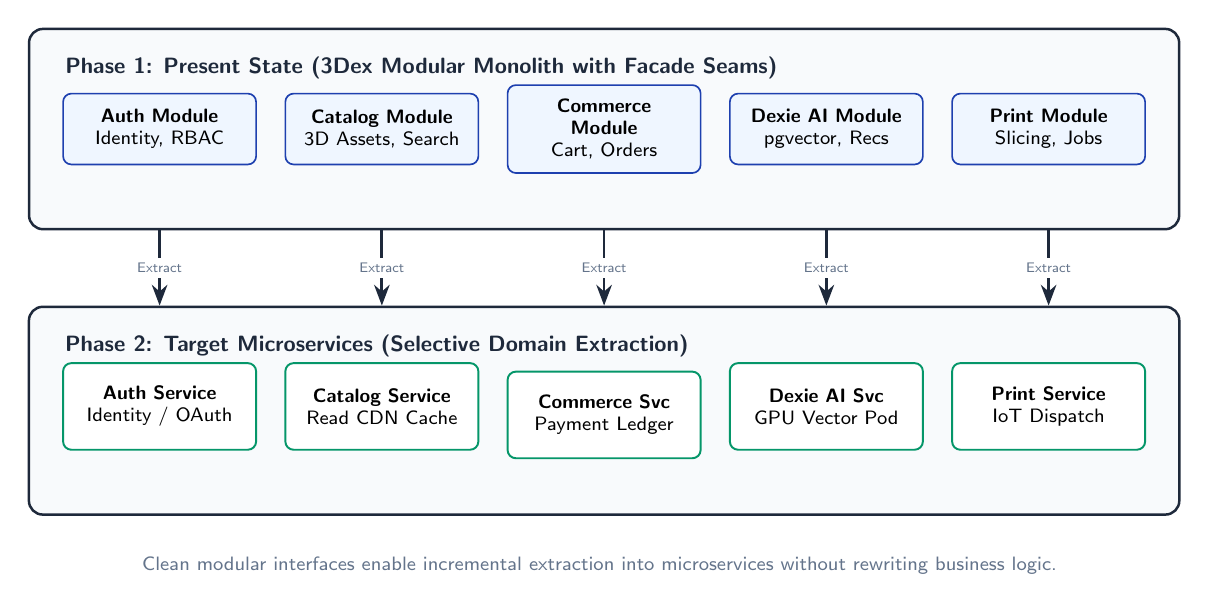
\begin{tikzpicture}[
    font=\small,
    >=Stealth,
    node distance=0.4cm and 0.4cm,
    modbox/.style={
        draw=cblue,
        fill=cbluelight,
        rounded corners=3pt,
        line width=0.6pt,
        align=center,
        inner sep=5pt,
        font=\scriptsize,
        text width=2.1cm,
        minimum height=0.9cm
    },
    svcbox/.style={
        draw=cgreen,
        fill=white,
        rounded corners=3pt,
        line width=0.7pt,
        align=center,
        inner sep=5pt,
        font=\scriptsize,
        text width=2.1cm,
        minimum height=1.1cm
    },
    flow/.style={
        ->,
        line width=1pt,
        draw=cborder
    }
]

    % Phase 1: Modules
    \node[modbox] (m_auth) {\textbf{Auth Module}\\Identity, RBAC};
    \node[modbox, right=0.35cm of m_auth] (m_cat) {\textbf{Catalog Module}\\3D Assets, Search};
    \node[modbox, right=0.35cm of m_cat] (m_com) {\textbf{Commerce Module}\\Cart, Orders};
    \node[modbox, right=0.35cm of m_com] (m_dex) {\textbf{Dexie AI Module}\\pgvector, Recs};
    \node[modbox, right=0.35cm of m_dex] (m_prt) {\textbf{Print Module}\\Slicing, Jobs};

    % Phase 1 Container
    \begin{scope}[on background layer]
        \node[draw=cborder, fill=cbg, rounded corners=5pt, line width=0.9pt,
              fit=(m_auth) (m_cat) (m_com) (m_dex) (m_prt),
              inner xsep=12pt, inner ysep=20pt] (mono_box) {};
    \end{scope}

    \node[anchor=north west, font=\bfseries\footnotesize, text=cborder] at (mono_box.north west) [xshift=10pt, yshift=-7pt] {
        Phase 1: Present State (3Dex Modular Monolith with Facade Seams)
    };

    % Phase 2: Microservices positioned with clear vertical separation (2.4cm)
    \node[svcbox, below=2.5cm of m_auth] (s_auth) {\textbf{Auth Service}\\Identity / OAuth};
    \node[svcbox, below=2.5cm of m_cat] (s_cat) {\textbf{Catalog Service}\\Read CDN Cache};
    \node[svcbox, below=2.5cm of m_com] (s_com) {\textbf{Commerce Svc}\\Payment Ledger};
    \node[svcbox, below=2.5cm of m_dex] (s_dex) {\textbf{Dexie AI Svc}\\GPU Vector Pod};
    \node[svcbox, below=2.5cm of m_prt] (s_prt) {\textbf{Print Service}\\IoT Dispatch};

    % Phase 2 Container
    \begin{scope}[on background layer]
        \node[draw=cborder, fill=cbg, rounded corners=5pt, line width=0.9pt,
              fit=(s_auth) (s_cat) (s_com) (s_dex) (s_prt),
              inner xsep=12pt, inner ysep=20pt] (micro_box) {};
    \end{scope}

    \node[anchor=north west, font=\bfseries\footnotesize, text=cborder] at (micro_box.north west) [xshift=10pt, yshift=-7pt] {
        Phase 2: Target Microservices (Selective Domain Extraction)
    };

    % Extraction arrows going across the clear gap
    \draw[flow] (mono_box.south -| m_auth) -- (micro_box.north -| s_auth)
        node[midway, fill=white, inner sep=2pt, font=\tiny, text=cgray] {Extract};
    \draw[flow] (mono_box.south -| m_cat) -- (micro_box.north -| s_cat)
        node[midway, fill=white, inner sep=2pt, font=\tiny, text=cgray] {Extract};
    \draw[flow] (mono_box.south -| m_com) -- (micro_box.north -| s_com)
        node[midway, fill=white, inner sep=2pt, font=\tiny, text=cgray] {Extract};
    \draw[flow] (mono_box.south -| m_dex) -- (micro_box.north -| s_dex)
        node[midway, fill=white, inner sep=2pt, font=\tiny, text=cgray] {Extract};
    \draw[flow] (mono_box.south -| m_prt) -- (micro_box.north -| s_prt)
        node[midway, fill=white, inner sep=2pt, font=\tiny, text=cgray] {Extract};

    % Footnote
    \node[below=0.4cm of micro_box, font=\scriptsize, align=center, text=cgray] {
        Clean modular interfaces enable incremental extraction into microservices without rewriting business logic.
    };

\end{tikzpicture}
\end{document}
